\subsection{Phát Hiện Vi Phạm}
% -----------------------------------------------------------------------------

Không có công cụ đơn lẻ nào đủ trong hồi quy bội. Năm công cụ sau được dùng theo thứ tự, từ khảo sát ban đầu đến xác nhận hình thức.

\begin{center}
\begin{tabular}{@{}llp{6.2cm}@{}}
\toprule
\textbf{Công cụ} & \textbf{Khi dùng} & \textbf{Phát hiện} \\
\midrule
Ma trận đồ thị phân tán   & Trước khi khớp  & Độ cong biên rõ ràng \\
Phần dư theo giá trị khớp & Sau khi khớp    & Có gì đó sai tổng thể \\
Phần dư theo từng $X_j$   & Sau khi khớp    & Biến nào là nguồn gốc \\
Đồ thị hồi quy riêng phần & Sau khi khớp    & Đóng góp tuyến tính riêng biệt của từng biến \\
Kiểm định Tukey            & Sau khi đồ thị gợi ý & Xác nhận hình thức về độ cong \\
\bottomrule
\end{tabular}
\end{center}

% - - - - - - - - - - - - - - - - - - - - - - - - - - - - - - - - - - - - - -
\subsubsection{Ma Trận Đồ Thị Phân Tán}

Vẽ mọi cặp quan hệ giữa $Y$ và các biến dự báo $X_1, \ldots, X_k$ trong một lưới trước khi khớp bất cứ thứ gì. Cho thấy bức tranh trực quan về các mối quan hệ biên và có thể báo hiệu độ cong rõ ràng ngay từ đầu.

\textbf{Giới hạn:} Chỉ nắm bắt quan hệ hai biến. Phi tuyến chỉ xuất hiện trong sự kết hợp của nhiều biến sẽ ẩn ở đây. Không thay thế được các công cụ sau khi khớp.

\begin{figure}[H]
  \centering
  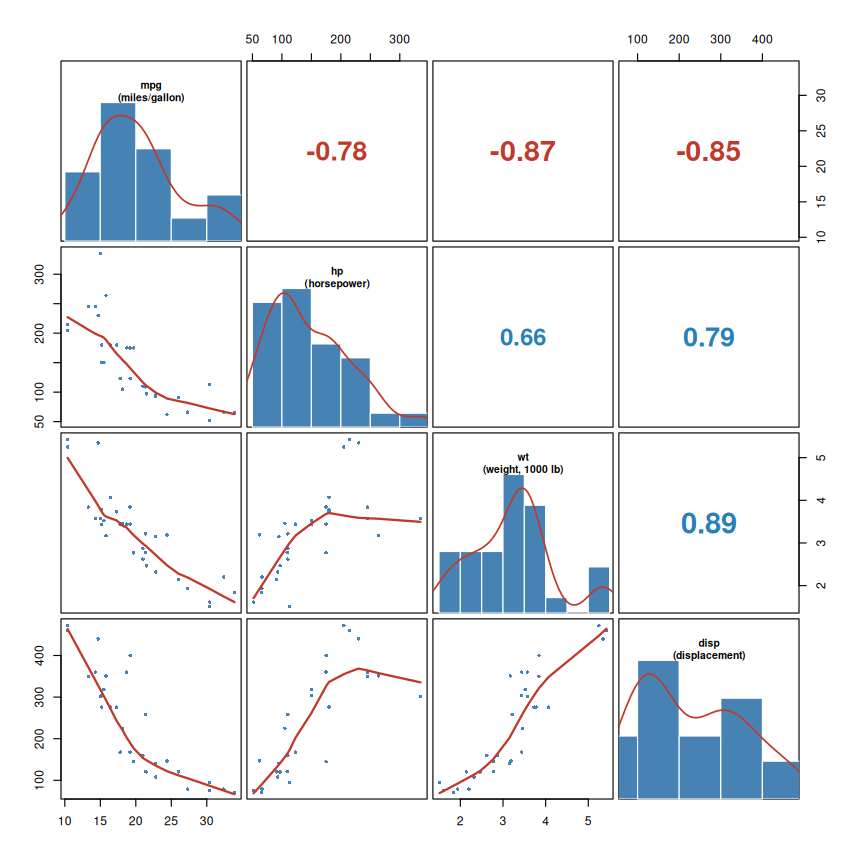
\includegraphics[width=0.88\textwidth]{./figures/fig14_scatterplot_matrix.png}
  \caption{Ma trận đồ thị phân tán cho bốn biến của \texttt{mtcars}.
  \textbf{Tam giác dưới:} scatter plot với đường LOESS (đỏ)---cho thấy độ cong biên trước khi khớp mô hình.
  \textbf{Đường chéo:} histogram mật độ của từng biến riêng lẻ.
  \textbf{Tam giác trên:} hệ số tương quan Pearson (cỡ chữ theo độ lớn, xanh dương = dương, đỏ = âm).
  Quan hệ \texttt{mpg}--\texttt{hp} và \texttt{mpg}--\texttt{disp} có đường LOESS cong rõ---gợi ý phi tuyến biên cần kiểm tra kỹ hơn sau khi khớp.}
  \label{fig:scattermat}
\end{figure}

\begin{lstlisting}[style=Rstyle]
# Ma tran do thi phan tan co LOESS va tuong quan
panel_scatter <- function(x, y, ...) {
  points(x, y, pch = 16, cex = 0.65, col = "steelblue")
  lines(lowess(x, y), col = "red", lwd = 2)
}
panel_cor <- function(x, y, ...) {
  r <- cor(x, y, use = "complete.obs")
  text(0.5, 0.5, round(r, 2), cex = 0.8 + 1.8*abs(r),
       col = if(r > 0) "blue" else "red", font = 2,
       transform = NULL)
}
pairs(mtcars[, c("mpg", "hp", "wt", "disp")],
      lower.panel = panel_scatter,
      upper.panel = panel_cor)
\end{lstlisting}

% - - - - - - - - - - - - - - - - - - - - - - - - - - - - - - - - - - - - - -
\subsubsection{Phần Dư Theo Giá Trị Khớp (Công Cụ Chính)}

Trục $x$ là giá trị khớp $\hat{y}$, trục $y$ là phần dư $e_i = y_i - \hat{y}_i$. Công cụ này hoạt động như ``kính lúp'': trừ đi xu hướng tuyến tính, phóng đại những sai lệch nhỏ bên dưới.

\begin{itemize}
  \item \textbf{Không vi phạm:} Điểm phân tán ngẫu nhiên quanh $y = 0$, đường LOESS nằm ngang---đây là ``biểu đồ rỗng'' lý tưởng.
  \item \textbf{Vi phạm:} Đường LOESS tạo thành dạng cong (chữ U, chữ S): quan hệ phi tuyến bị bỏ sót ở đâu đó trong mô hình.
\end{itemize}

Trong hồi quy bội, đồ thị này chỉ báo ``có điều gì đó sai'' nhưng không chỉ ra biến nào là nguyên nhân.

\begin{figure}[H]
  \centering
  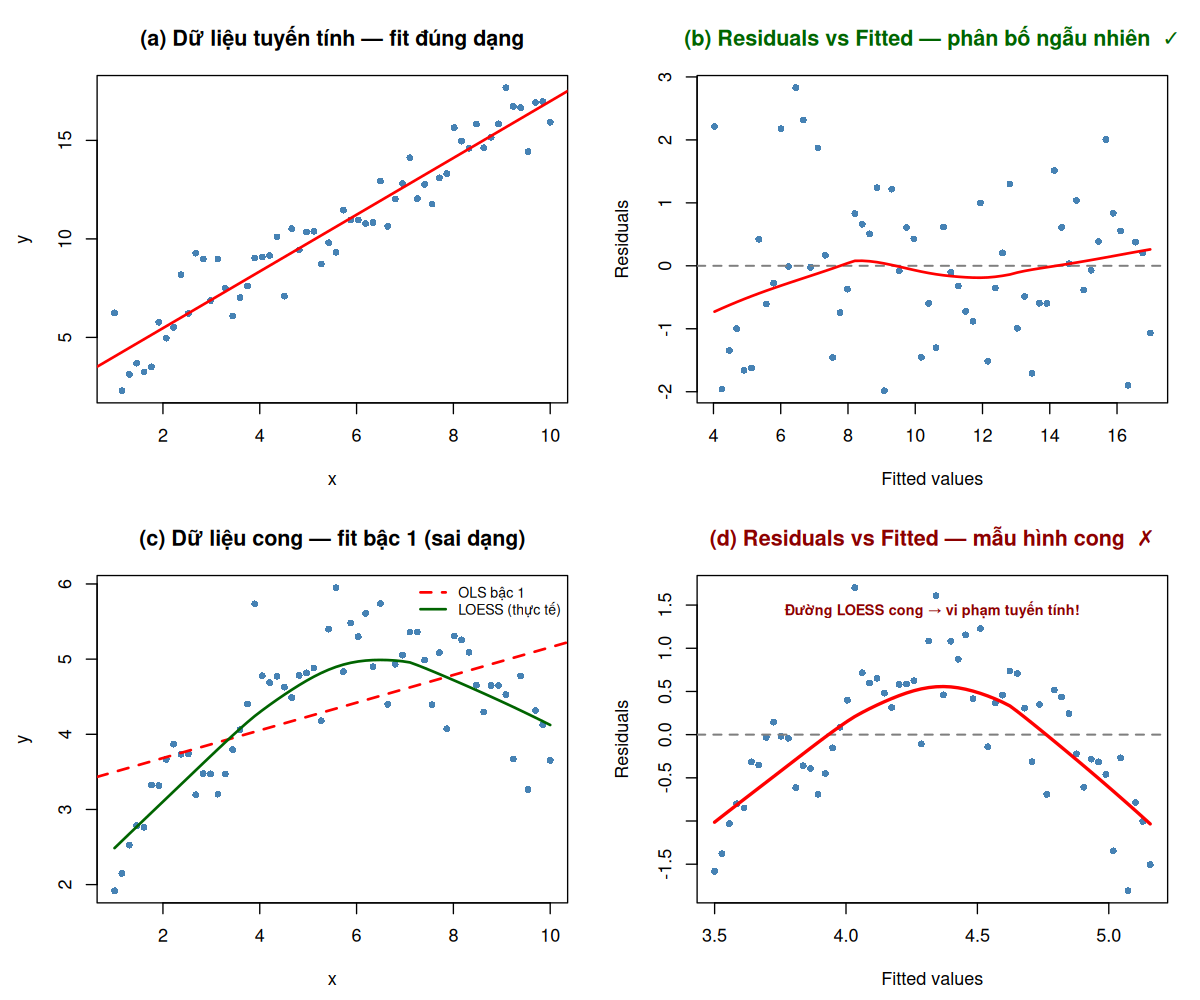
\includegraphics[width=\textwidth]{./figures/fig3_residual_plots.png}
  \caption{Đồ thị phần dư theo giá trị khớp: ``biểu đồ rỗng'' (không vi phạm) so với mẫu hình cong (vi phạm).
  \textbf{(a)--(b)} Dữ liệu tuyến tính: LOESS gần nằm ngang, điểm phân tán đều.
  \textbf{(c)--(d)} Dữ liệu cong khớp bằng bậc 1: LOESS cong hình chữ U xác nhận vi phạm tuyến tính.}
  \label{fig:residual_plots}
\end{figure}

% - - - - - - - - - - - - - - - - - - - - - - - - - - - - - - - - - - - - - -
\subsubsection{Phần Dư Theo Từng Biến Dự Báo}

Vẽ phần dư $e_i$ theo từng biến $X_j$ riêng lẻ. Dạng cong trong một trong các đồ thị này \textit{khoanh vùng vấn đề}: biến cụ thể đó không được mô hình hóa đúng dạng. Thường có thể khắc phục bằng cách thêm số hạng $X_j^2$ hoặc $\log X_j$.

\begin{lstlisting}[style=Rstyle]
fit <- lm(mpg ~ hp + wt + disp, data = mtcars)
par(mfrow = c(1, 3))
for (v in c("hp", "wt", "disp")) {
  plot(mtcars[[v]], residuals(fit),
       xlab = v, ylab = "Residuals", pch = 16, col = "steelblue")
  abline(h = 0, lty = 2)
  lines(lowess(mtcars[[v]], residuals(fit)), col = "red", lwd = 2)
}
\end{lstlisting}

% - - - - - - - - - - - - - - - - - - - - - - - - - - - - - - - - - - - - - -
\subsubsection{Đồ Thị Hồi Quy Riêng Phần}
\label{sec:partial_reg}

Đồ thị phần dư theo từng $X_j$ có một điểm yếu: nó không loại trừ ảnh hưởng của các biến khác, nên có thể phản ánh sai mối quan hệ của $X_j$ với $Y$. Đồ thị hồi quy riêng phần (added-variable plot) khắc phục điều này.

\textbf{Cách xây dựng.} Cho biến dự báo $X_j$:
\begin{enumerate}
  \item Hồi quy $Y$ lên tất cả các biến trừ $X_j$ $\to$ lấy phần dư $e_Y$.
  \item Hồi quy $X_j$ lên tất cả các biến trừ $X_j$ $\to$ lấy phần dư $e_{X_j}$.
  \item Vẽ $e_Y$ theo $e_{X_j}$.
\end{enumerate}

Độ dốc của đồ thị này bằng \textit{chính xác} hệ số $\hat{\beta}_j$ trong mô hình đầy đủ---nó cô lập đóng góp tuyến tính \textit{duy nhất} của $X_j$ sau khi đã tính đến mọi biến khác. Dạng phi tuyến ở đây xác nhận $X_j$ không được đưa vào mô hình đúng dạng.

\begin{figure}[H]
  \centering
  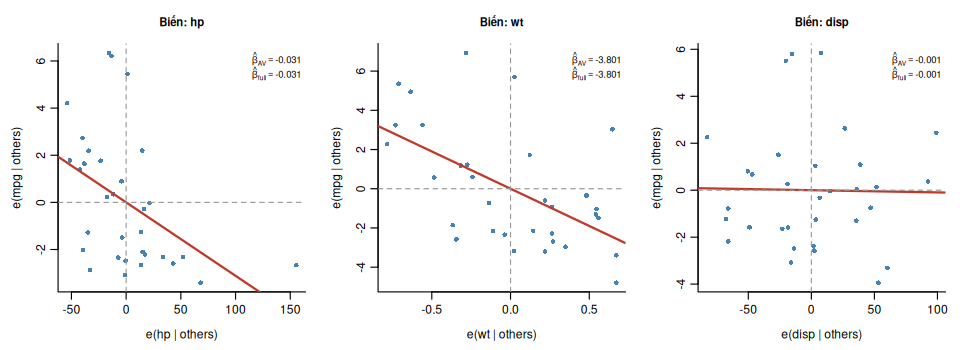
\includegraphics[width=\textwidth]{./figures/fig8_avplot.png}
  \caption{Đồ thị hồi quy riêng phần cho mô hình \texttt{mpg \textasciitilde{} hp + wt + disp} (mtcars).
  Trục $x$ và $y$ là phần dư của $X_j$ và $Y$ sau khi đã loại bỏ ảnh hưởng của các biến còn lại.
  Chú thích trên mỗi panel: $\hat{\beta}_{\text{AV}}$ (độ dốc của đồ thị) và $\hat{\beta}_{\text{full}}$ (hệ số trong mô hình đầy đủ)---hai giá trị khớp chính xác nhau.
  Quan hệ gần thẳng xác nhận dạng tuyến tính là phù hợp cho cả ba biến trong mô hình này.}
  \label{fig:avplot}
\end{figure}

\begin{lstlisting}[style=Rstyle]
# Implement added-variable plot thu cong (khong can package car)
av_plot <- function(fit, jname) {
  vars   <- attr(terms(fit), "term.labels")
  others <- setdiff(vars, jname)
  fmY    <- as.formula(paste("mpg ~",  paste(others, collapse = "+")))
  fmXj   <- as.formula(paste(jname,    "~", paste(others, collapse = "+")))
  eY     <- residuals(lm(fmY,  data = model.frame(fit)))
  eXj    <- residuals(lm(fmXj, data = model.frame(fit)))
  plot(eXj, eY, pch = 16, col = "steelblue",
       xlab = paste0("e(", jname, " | others)"),
       ylab = "e(mpg | others)", main = jname)
  abline(lm(eY ~ eXj), col = "red", lwd = 2)
}

fit_full <- lm(mpg ~ hp + wt + disp, data = mtcars)
par(mfrow = c(1, 3))
for (v in c("hp", "wt", "disp")) av_plot(fit_full, v)
\end{lstlisting}

% - - - - - - - - - - - - - - - - - - - - - - - - - - - - - - - - - - - - - -
\subsubsection{Kiểm Định Tukey Cho Tính Không Cộng Tính}

Khi đồ thị phần dư gợi ý độ cong, hình thức hóa ấn tượng thị giác: chọn một đại lượng $U$ (một biến dự báo cụ thể hoặc giá trị khớp $\hat{y}$), thêm $U^2$ làm số hạng phụ vào mô hình, và chạy kiểm định $t$ cho hệ số của nó:
\[
  Y = \beta_0 + \beta_1 X_1 + \cdots + \beta_p X_p + \gamma U^2 + \varepsilon,
  \qquad H_0{:}\ \gamma = 0
\]

Kết quả có ý nghĩa ($p < 0.05$) xác nhận độ cong có hệ thống. Khi $U = \hat{y}$, thủ tục này được gọi là \textbf{kiểm định Tukey cho tính không cộng tính}---nó kiểm tra một cách tổng quát xem có bất kỳ dạng phi tuyến nào bị bỏ sót trong mô hình hay không.

\begin{lstlisting}[style=Rstyle]
fit_base  <- lm(mpg ~ hp + wt, data = mtcars)
yhat      <- fitted(fit_base)

# Tukey's test: them yhat^2, kiem tra he so gamma
fit_tukey <- lm(mpg ~ hp + wt + I(yhat^2), data = mtcars)
summary(fit_tukey)$coefficients["I(yhat^2)", ]
\end{lstlisting}

\begin{lstlisting}[style=output]
              Estimate Std. Error   t value  Pr(>|t|)
I(yhat^2)  -0.0033021  0.0016574 -1.992     0.0560
\end{lstlisting}

$p = 0.056$ gần ngưỡng: đồ thị phần dư của mô hình \texttt{mpg \textasciitilde{} hp + wt} cho thấy độ cong nhẹ, kiểm định Tukey xác nhận đây không phải hoàn toàn ngẫu nhiên. Thêm \texttt{I(hp\^{}2)} hoặc dùng \texttt{poly(hp, 2)} sẽ giải quyết vấn đề.

% - - - - - - - - - - - - - - - - - - - - - - - - - - - - - - - - - - - - - -
\subsubsection{Đồ Thị Nền và Giao Thức Xếp Hàng}
% - - - - - - - - - - - - - - - - - - - - - - - - - - - - - - - - - - - - - -

Khi đọc đồ thị phần dư, mắt người dễ thấy ``mẫu hình'' ngay cả trong dữ liệu hoàn toàn ngẫu nhiên. Câu hỏi cần đặt ra: mẫu hình ta thấy là vi phạm thực sự hay chỉ là biến động tự nhiên?

Một \textbf{đồ thị nền} là đồ thị phần dư được tạo từ dữ liệu mô phỏng \textit{khi mô hình hoàn toàn đúng}---đây là chuẩn gốc của sự ngẫu nhiên với cỡ mẫu $n$ và $\hat{\sigma}$ cụ thể:
\begin{enumerate}
  \item Ước lượng mô hình gốc, thu được $\hat{\beta}$ và $\hat{\sigma}$.
  \item Mô phỏng: $y^* = X\hat{\beta} + \varepsilon^*$, $\varepsilon^* \sim \mathcal{N}(0, \hat{\sigma}^2)$.
  \item Khớp lại cùng mô hình trên $y^*$, lấy phần dư và vẽ đồ thị.
\end{enumerate}

\textbf{Giao thức xếp hàng} (Wickham et al., 2010) biến việc đọc đồ thị thành kiểm định thống kê thị giác: tạo $m-1$ đồ thị nền, chèn đồ thị thực vào vị trí ngẫu nhiên, hiển thị tất cả $m$ đồ thị. Nếu người quan sát xác định đúng đồ thị thực, $p\text{-value} = 1/m$.

\begin{lstlisting}[style=Rstyle]
generate_null_residuals <- function(model) {
  n     <- length(fitted(model))
  y_sim <- fitted(model) + rnorm(n, sd = sigma(model))
  fit_null <- update(model, y_sim ~ .)
  data.frame(fitted = fitted(fit_null), resid = residuals(fit_null))
}

set.seed(2025)
fit      <- lm(mpg ~ hp, data = mtcars)
real_pos <- sample(1:9, 1)
par(mfrow = c(3, 3), mar = c(3, 3, 2.5, 1))
for (i in 1:9) {
  d <- if (i == real_pos) data.frame(fitted = fitted(fit),
                                      resid  = residuals(fit))
       else generate_null_residuals(fit)
  plot(d$fitted, d$resid, pch = 16, cex = 0.7, col = "steelblue",
       xlab = "Fitted", ylab = "Residuals", main = paste("Plot", i))
  abline(h = 0, lty = 2, col = "gray60")
  lines(lowess(d$fitted, d$resid), col = "red", lwd = 2)
}
\end{lstlisting}

\begin{figure}[H]
  \centering
  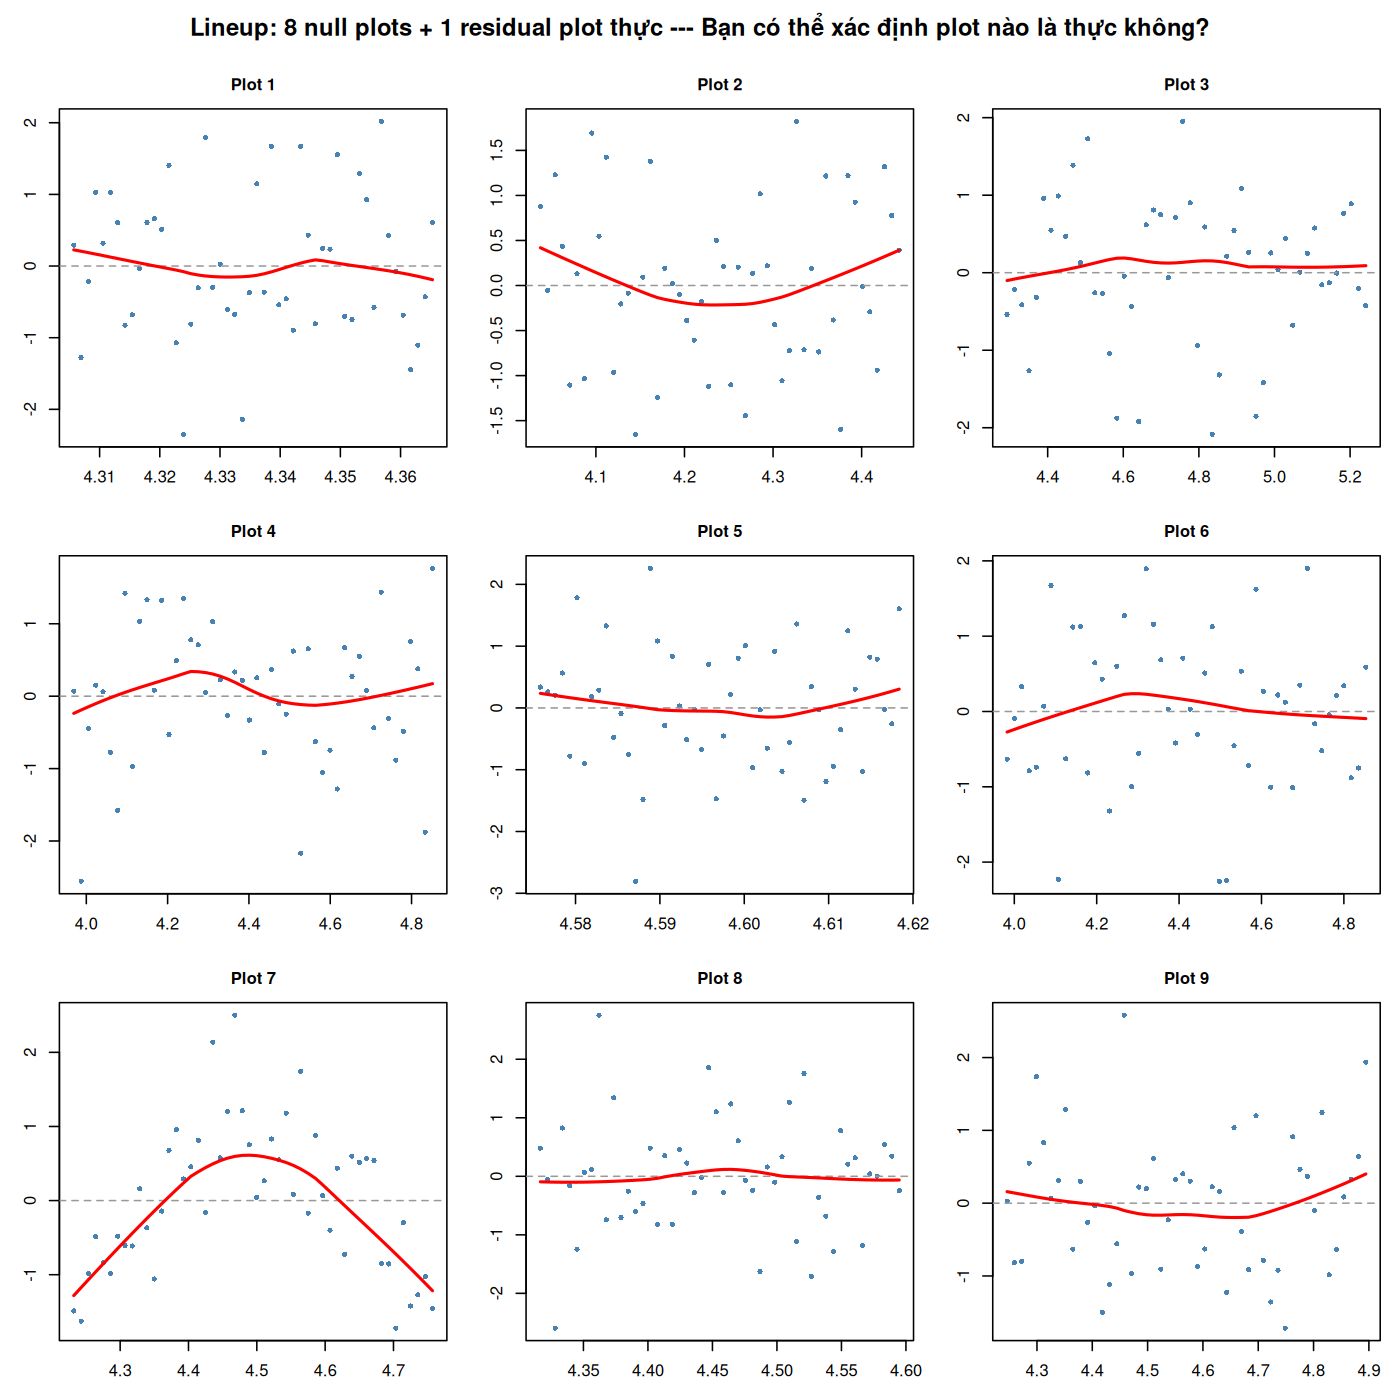
\includegraphics[width=\textwidth]{./figures/fig5_lineup.png}
  \caption{Giao thức xếp hàng: 8 đồ thị nền và 1 đồ thị phần dư thực (mô hình bậc 1 trên dữ liệu cong).
  Xác suất đoán ngẫu nhiên đúng là $1/9 \approx 11\%$. Nếu bạn nhận ra đồ thị thực, đó là bằng chứng thị giác có ý nghĩa thống kê.
  \textbf{Hữu ích nhất} khi $n < 30$ và mẫu hình phần dư mơ hồ.
  \textit{(Đáp án: Đồ thị 7.)}}
  \label{fig:lineup}
\end{figure}

% - - - - - - - - - - - - - - - - - - - - - - - - - - - - - - - - - - - - - -
\subsubsection{Phần Dư Chuẩn Hóa}
\label{sec:partial_reg}
% - - - - - - - - - - - - - - - - - - - - - - - - - - - - - - - - - - - - - -

Phần dư nguyên bản $e_i$ có phương sai không đồng nhất, phụ thuộc vào đòn bẩy $h_{ii}$:
\[
  \mathrm{Var}(e_i) = \sigma^2(1 - h_{ii})
\]

Tại điểm có đòn bẩy cao ($h_{ii}$ lớn), phần dư bị kéo về gần $0$ ngay cả khi mô hình sai---\textbf{hiệu ứng che khuất}. Nên dùng phần dư Student hóa ngoài \texttt{rstudent(model)} thay thế: chúng có phương sai đồng nhất và nhạy hơn với bất thường cục bộ. Đồ thị hồi quy riêng phần (mục~\ref{sec:partial_reg}) bổ sung góc nhìn cục bộ cho từng biến; hai công cụ bổ trợ nhau, không thay thế nhau.

% -----------------------------------------------------------------------------
